%%%%
%% Development
%%%
\chapter{Development}
\label{cha:development}

The development phase was split across three `iterations'. Each iteration would
add and improve upon existing functionality. In order to keep the documentation
as compact as possible, this chapter will only focus upon the final development 
phase. This will ensure that the contents of this chapter is in line with the 
latest development phase and source code.

This chapter will focus upon the user interface development and how it interacts
with the Java Servlets. There will also be signification focus upon the `back 
end' system, including how a clue is solved and how the solvers interact with 
various resources such as dictionaries and thesauri. 

Finally the overall system architecture will be discussed, proving an insight 
into it's development and how it has added to the overall product.

% User Interface Development Details
\newpage
%%%%
%% Design :: User Interface
%%%
\section{User Interface}
\label{sec:design_user_interface}

The previous sections have presented a number of system designs from a 
programmatic point of view. Within this section, there will be a focus upon 
user interface designs, and thus how the end user will interact with the system.

Fundamentally there are two aspects to the user interface design of the system 
--- inputting the clue and retrieving the results. Each of these aspects will 
be discussed in more detail in the following subsections.


%%%
%% Design :: User Interface :: Platform Support
%%%
\subsection{Platform Support} 
\label{sub:platform_support}

One of the main objective of the project is to develop a system that can be used
upon a number of mobile platforms, as well as trying not to neglect 
`traditional' desktop users.

In order to complete both of these objectives, a responsive design is required.
A responsive design is one that is able to dynamically change based upon the 
screen size.

This means that there will only be one code based for multiple screen sizes, and
thus allowing for increases in maintainability. All of the designs within this
section feature a responsive design. Figure \ref{fig:input_form_compare} 
illustrates the power of responsive designs.

The left-hand side form shows a `traditional' desktop experience, whilst the 
form upon the right-hand side, shows a mobile experience.

\begin{figure}[H]
  \centering
  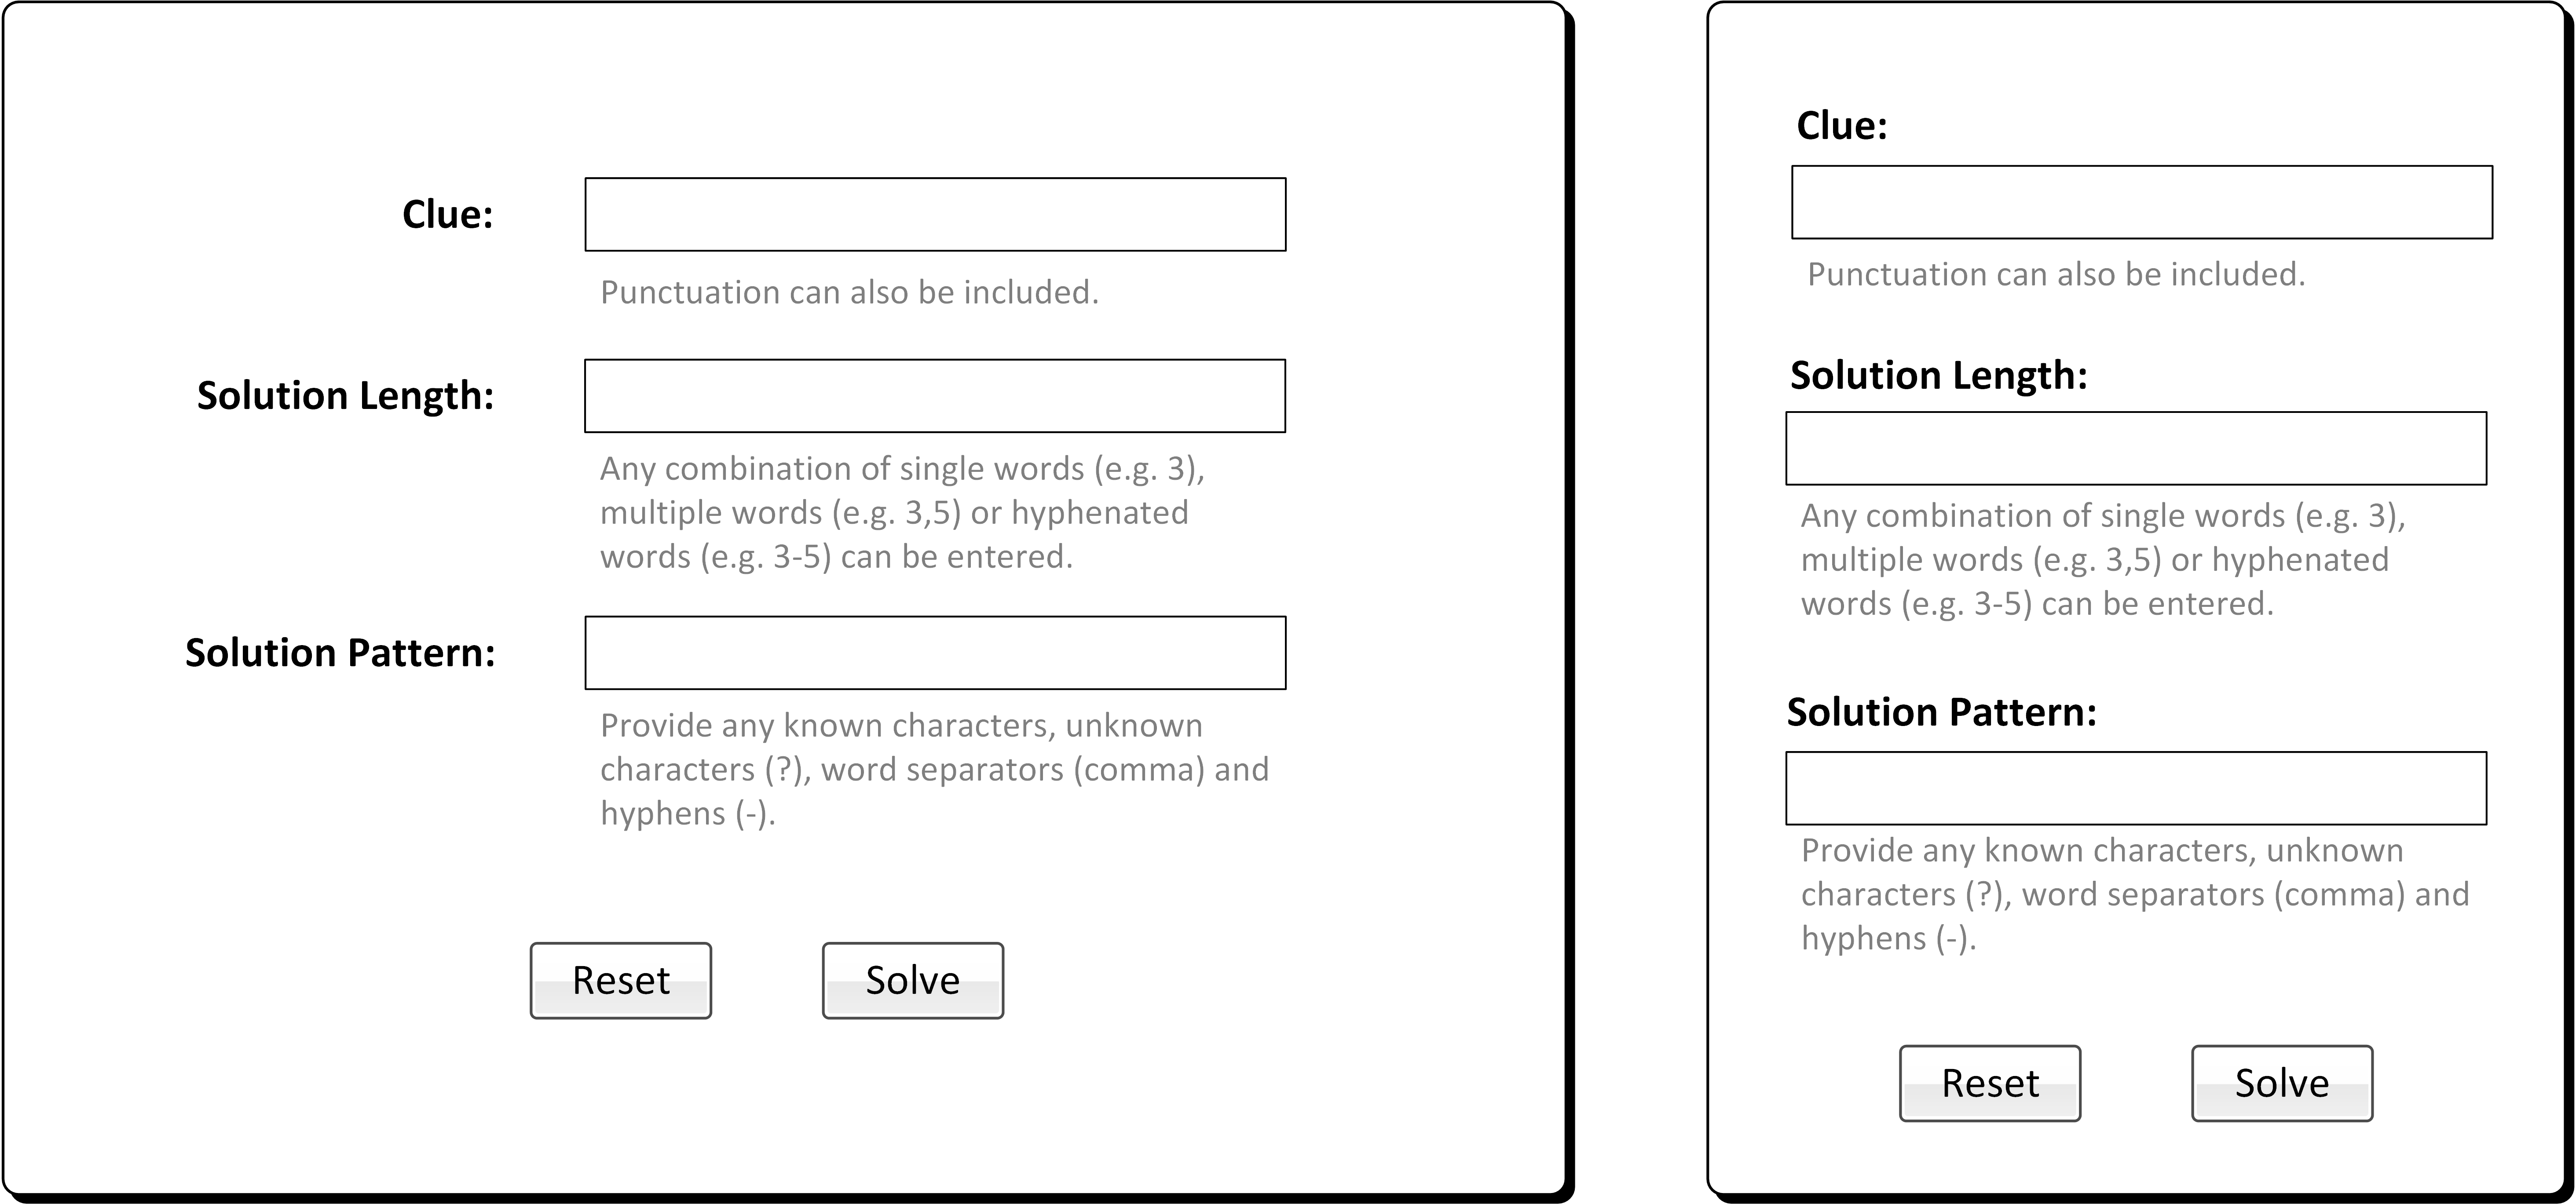
\includegraphics[width=0.8\textwidth]{design/ui/form_comparison.jpg}
  \caption{The input form to be completed by the end user}
  \label{fig:input_form_compare}
\end{figure}


%%%
%%  Design :: User Interface :: User Input
%%%
\subsection{User Input} 
\label{sub:user_input}

In order for the system to solve the clue, it must first be given the clue, 
along with additional supporting information. The additional information such as 
the solution length and pattern is vital to the system in order for it to 
compute the correct answer. 

However the intended users of the system are likely to be operating upon some 
form of mobile device, meaning that a simple and power interface is required. It
also means that space will be at a premium, and thus it can not afford to be 
wasted.

Figure \ref{fig:input_form} illustrates the design of the user input form. One 
of the most noticeable elements to the form design is how much space has been 
allocated to the input boxes. 

The design of the inputs utilises a bi-column setup using the ratio of 1:3. This
means that for every 1 pixel of space allocated to the left-hand labels, there 
will be 3 pixels of space allocated to the right-hand input boxes. This allows 
users of mobile devices to quickly select the input box, rather than having to 
tap a small area several times.

In order to assist the end user additional help blocks will be included, and 
give useful information to the user, such as describing the solution pattern 
format required.

\begin{figure}[H]
  \centering
  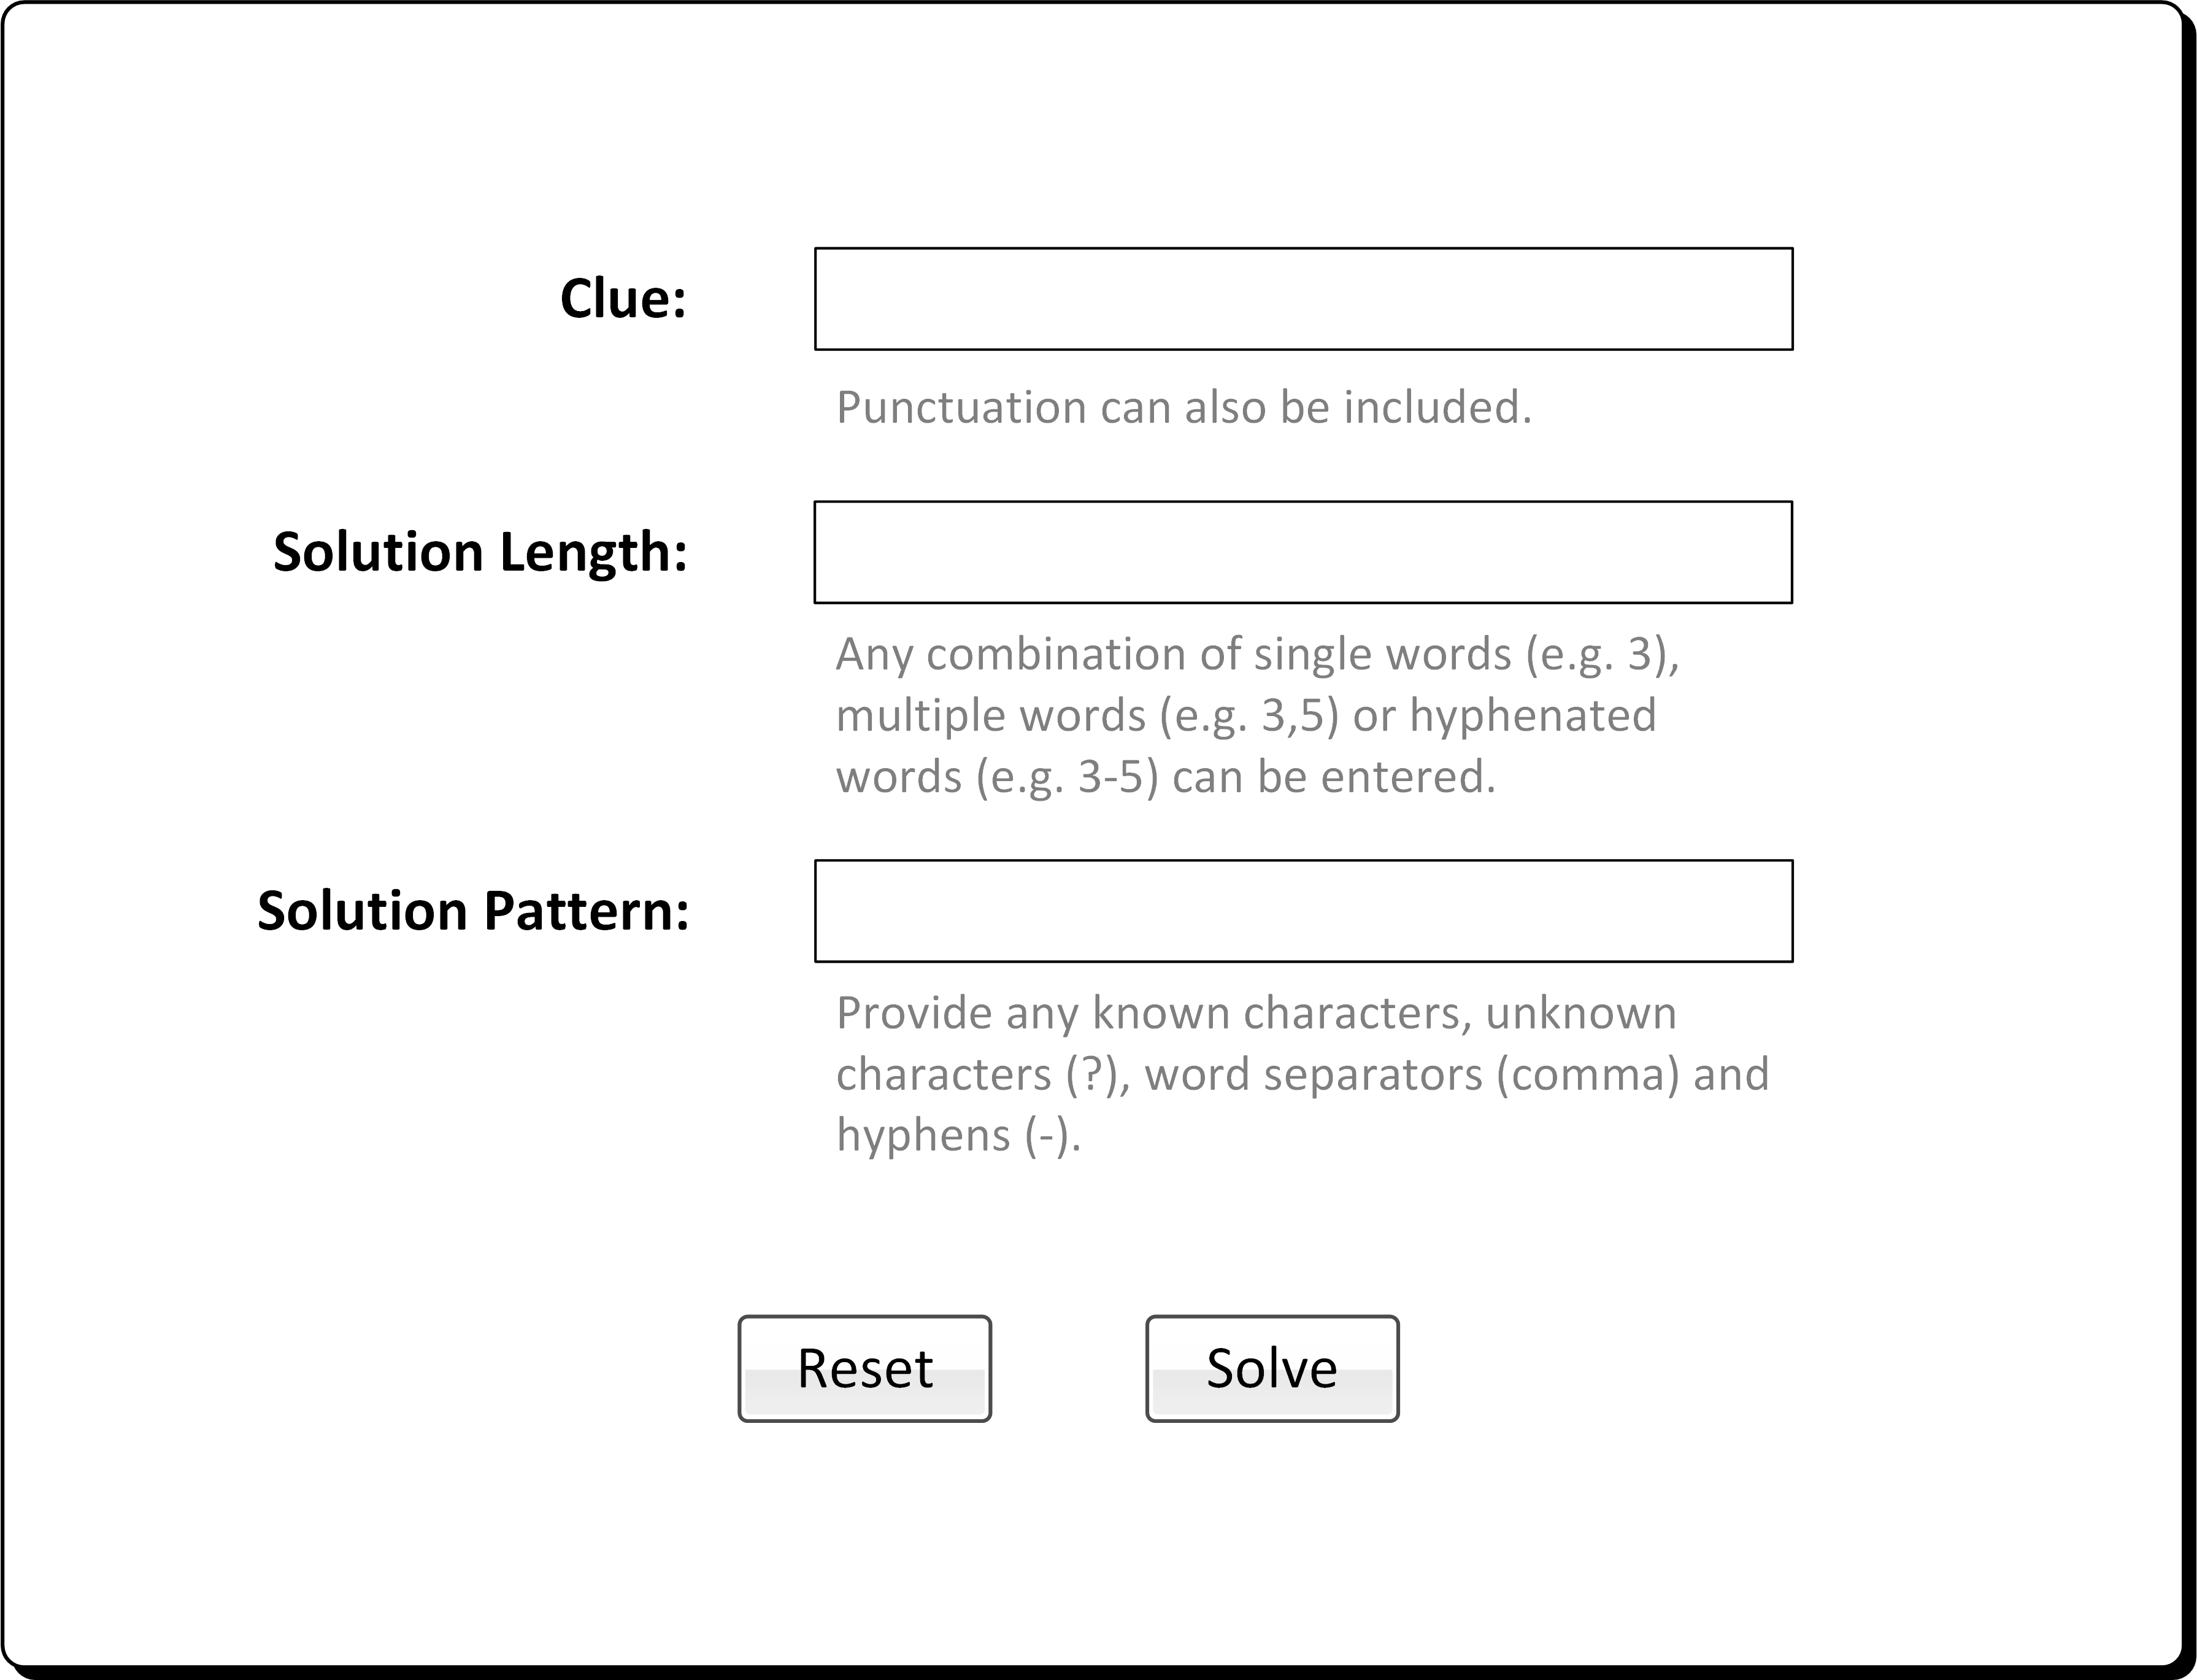
\includegraphics[width=0.8\textwidth]{design/ui/form.jpg}
  \caption{The input form to be completed by the end user}
  \label{fig:input_form}
\end{figure}

As the system is dealing with input from users, it is inevitable that a user 
will attempt to input incorrect data. This will require validation to be 
performed, and if validation has failed then the user should be notified. 

As previously mentioned space is a premium upon a mobile device. Therefore 
displaying a list of validation error messages at the top of the screen would 
not be utilising limited amount of space wisely.

In order to combat this issue, validation will be displayed `inline' with the 
form input elements, as seen within figure \ref{fig:input_form_error}. By 
utilising an `inline' approach it recycles the screen space that has been made 
available by the form.

For validations that have passed the input outline will change to green, and for
validations that have failed the input group will change to red. This will 
immediately alert the user to the various issues, and thus allows the user to 
fix the errors in a quicker and more efficient manner.

\begin{figure}[H]
  \centering
  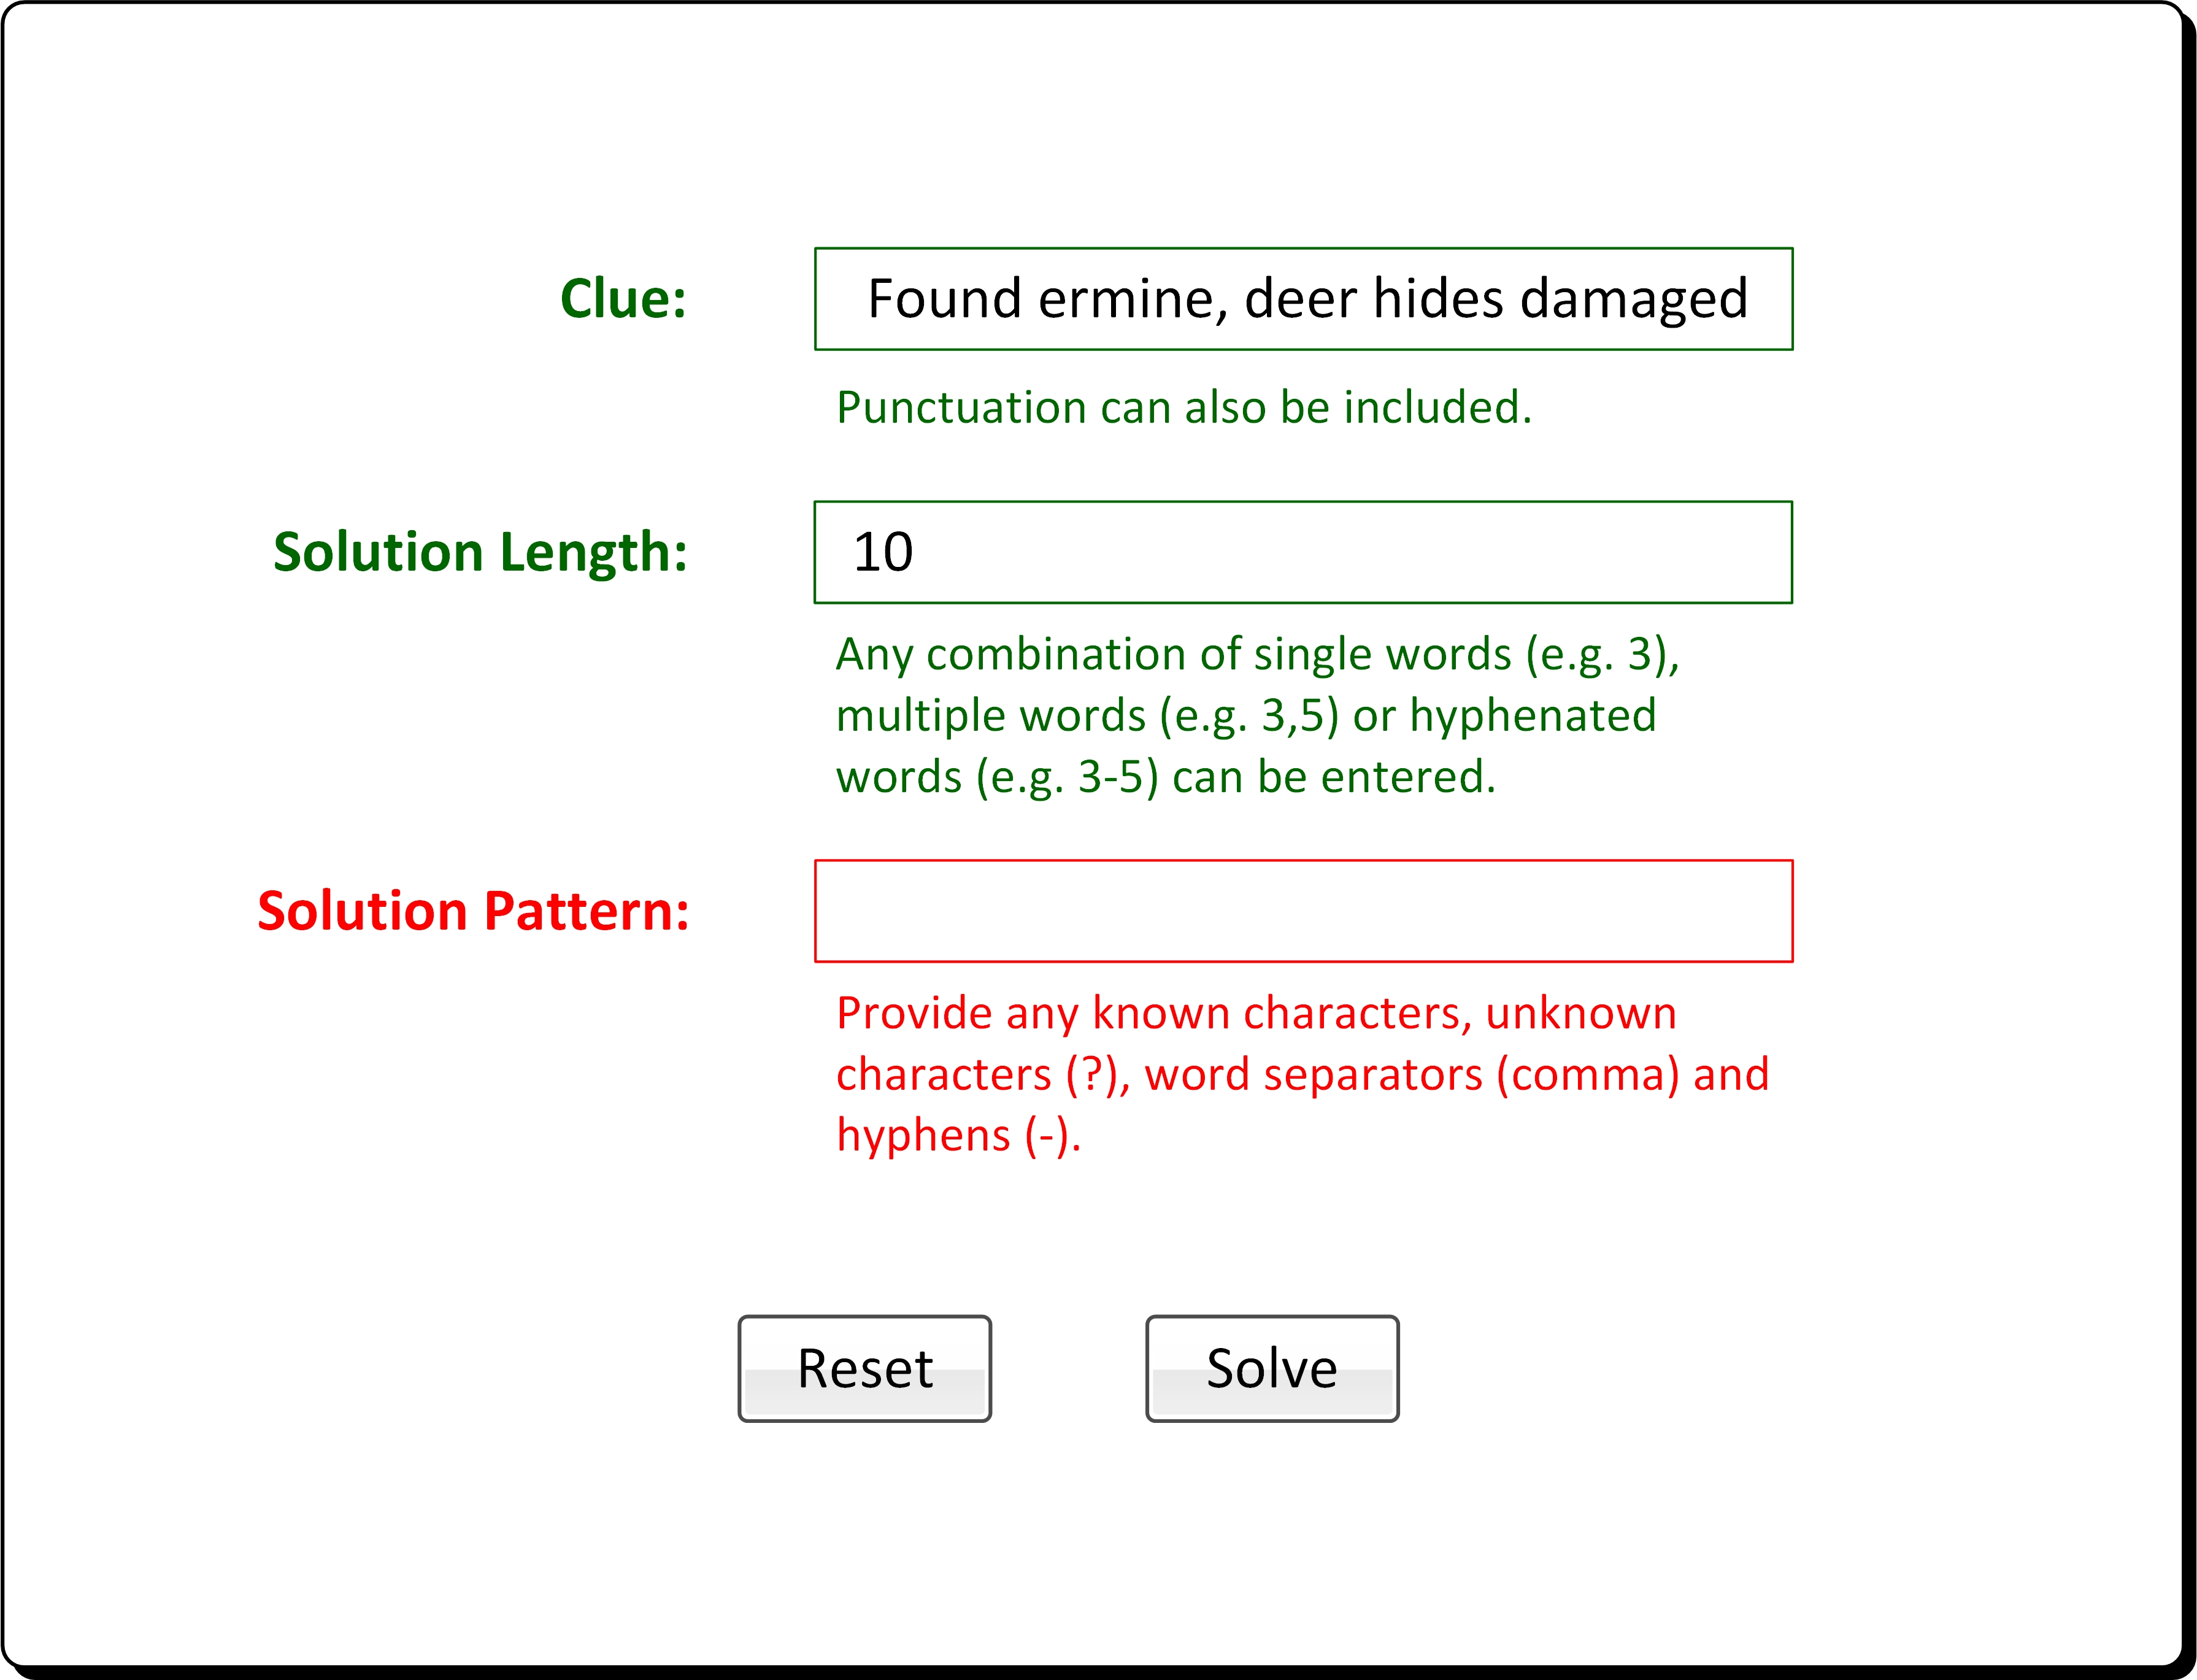
\includegraphics[width=0.8\textwidth]{design/ui/form_error.jpg}
  \caption{The input form indicating a validation error}
  \label{fig:input_form_error}
\end{figure}


%%%
%% Design :: User Interface :: Results
%%%
\subsection{Results} 
\label{sub:results}

The displaying of the results follows on from some of the previous design 
decisions. Each potential solution is rendered into it's own panel, and will 
contain the confidence rating, and the solver type that managed to deduce the 
solution (as shown in Figure \ref{fig:results_primary}).

Within an open panel, additional information is displayed --- known as the 
solution trace. A solution trace provides a step by step account of how the 
solution was able to be computed. The solution trace may help to teach users how
a particular type of clue is solved.

The results are order by confidence rating in ascending order, and by default 
the first panel will be `open', showing the solution trace. The reason for this
is that the top answer is likely to be the answer the end user is looking for

\begin{figure}[H]
  \centering
  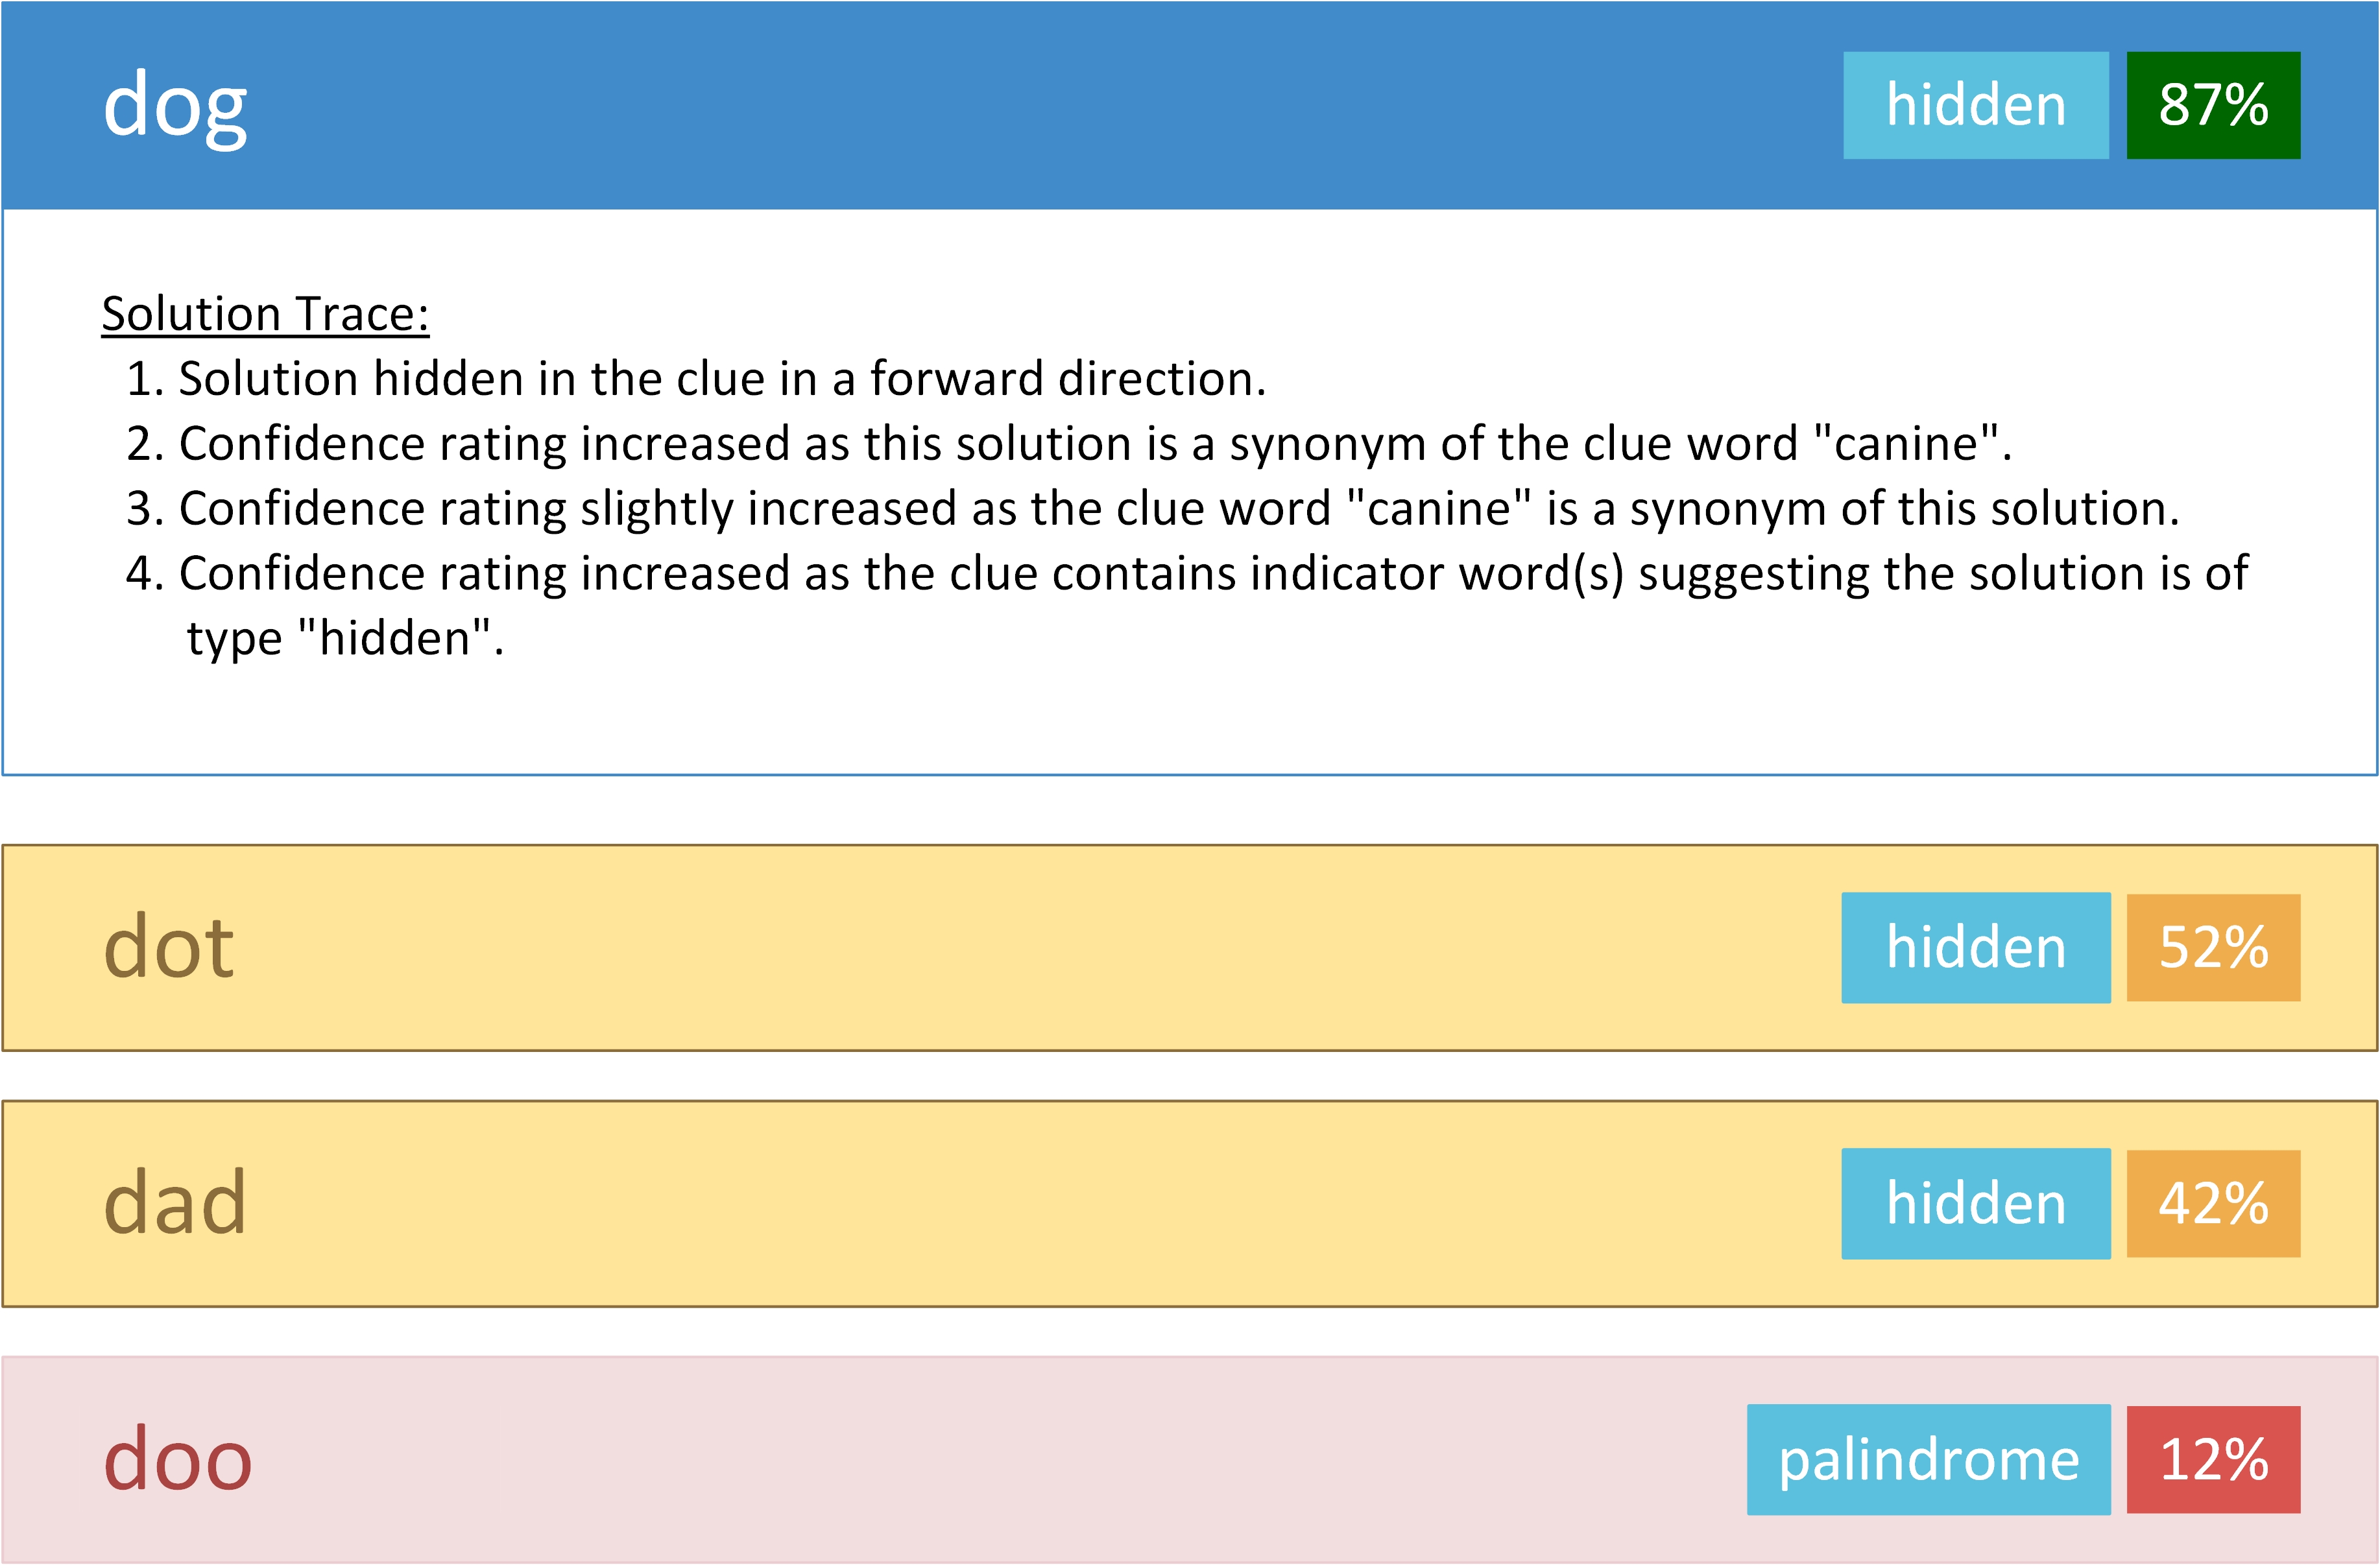
\includegraphics[width=0.8\textwidth]{design/ui/results_primary.jpg}
  \caption{Results list displaying the top answer in blue}
  \label{fig:results_primary}
\end{figure}

Each of the panels are ``clickable'', meaning that if any given panel is 
selected then the solution trace will be displayed, whilst previously selected 
panels will be `closed' (as shown in Figure \ref{fig:results_secondary}). The 
main reason behind this is to reduce the amount of scrolling a user has to do, 
especially for those without a mouse.

Each solution is awarded a colour based upon the confidence rating. Blue refers 
to a top answer, whilst the remaining colours (green, yellow and red) indicate 
the likely hood of the solution being correct. 

This will allow the end user to immediately deduce that `green' results are 
more likely to be correct in comparison to `red results', and that a `blue' 
result is likely to be correct.

\begin{figure}[H]
  \centering
  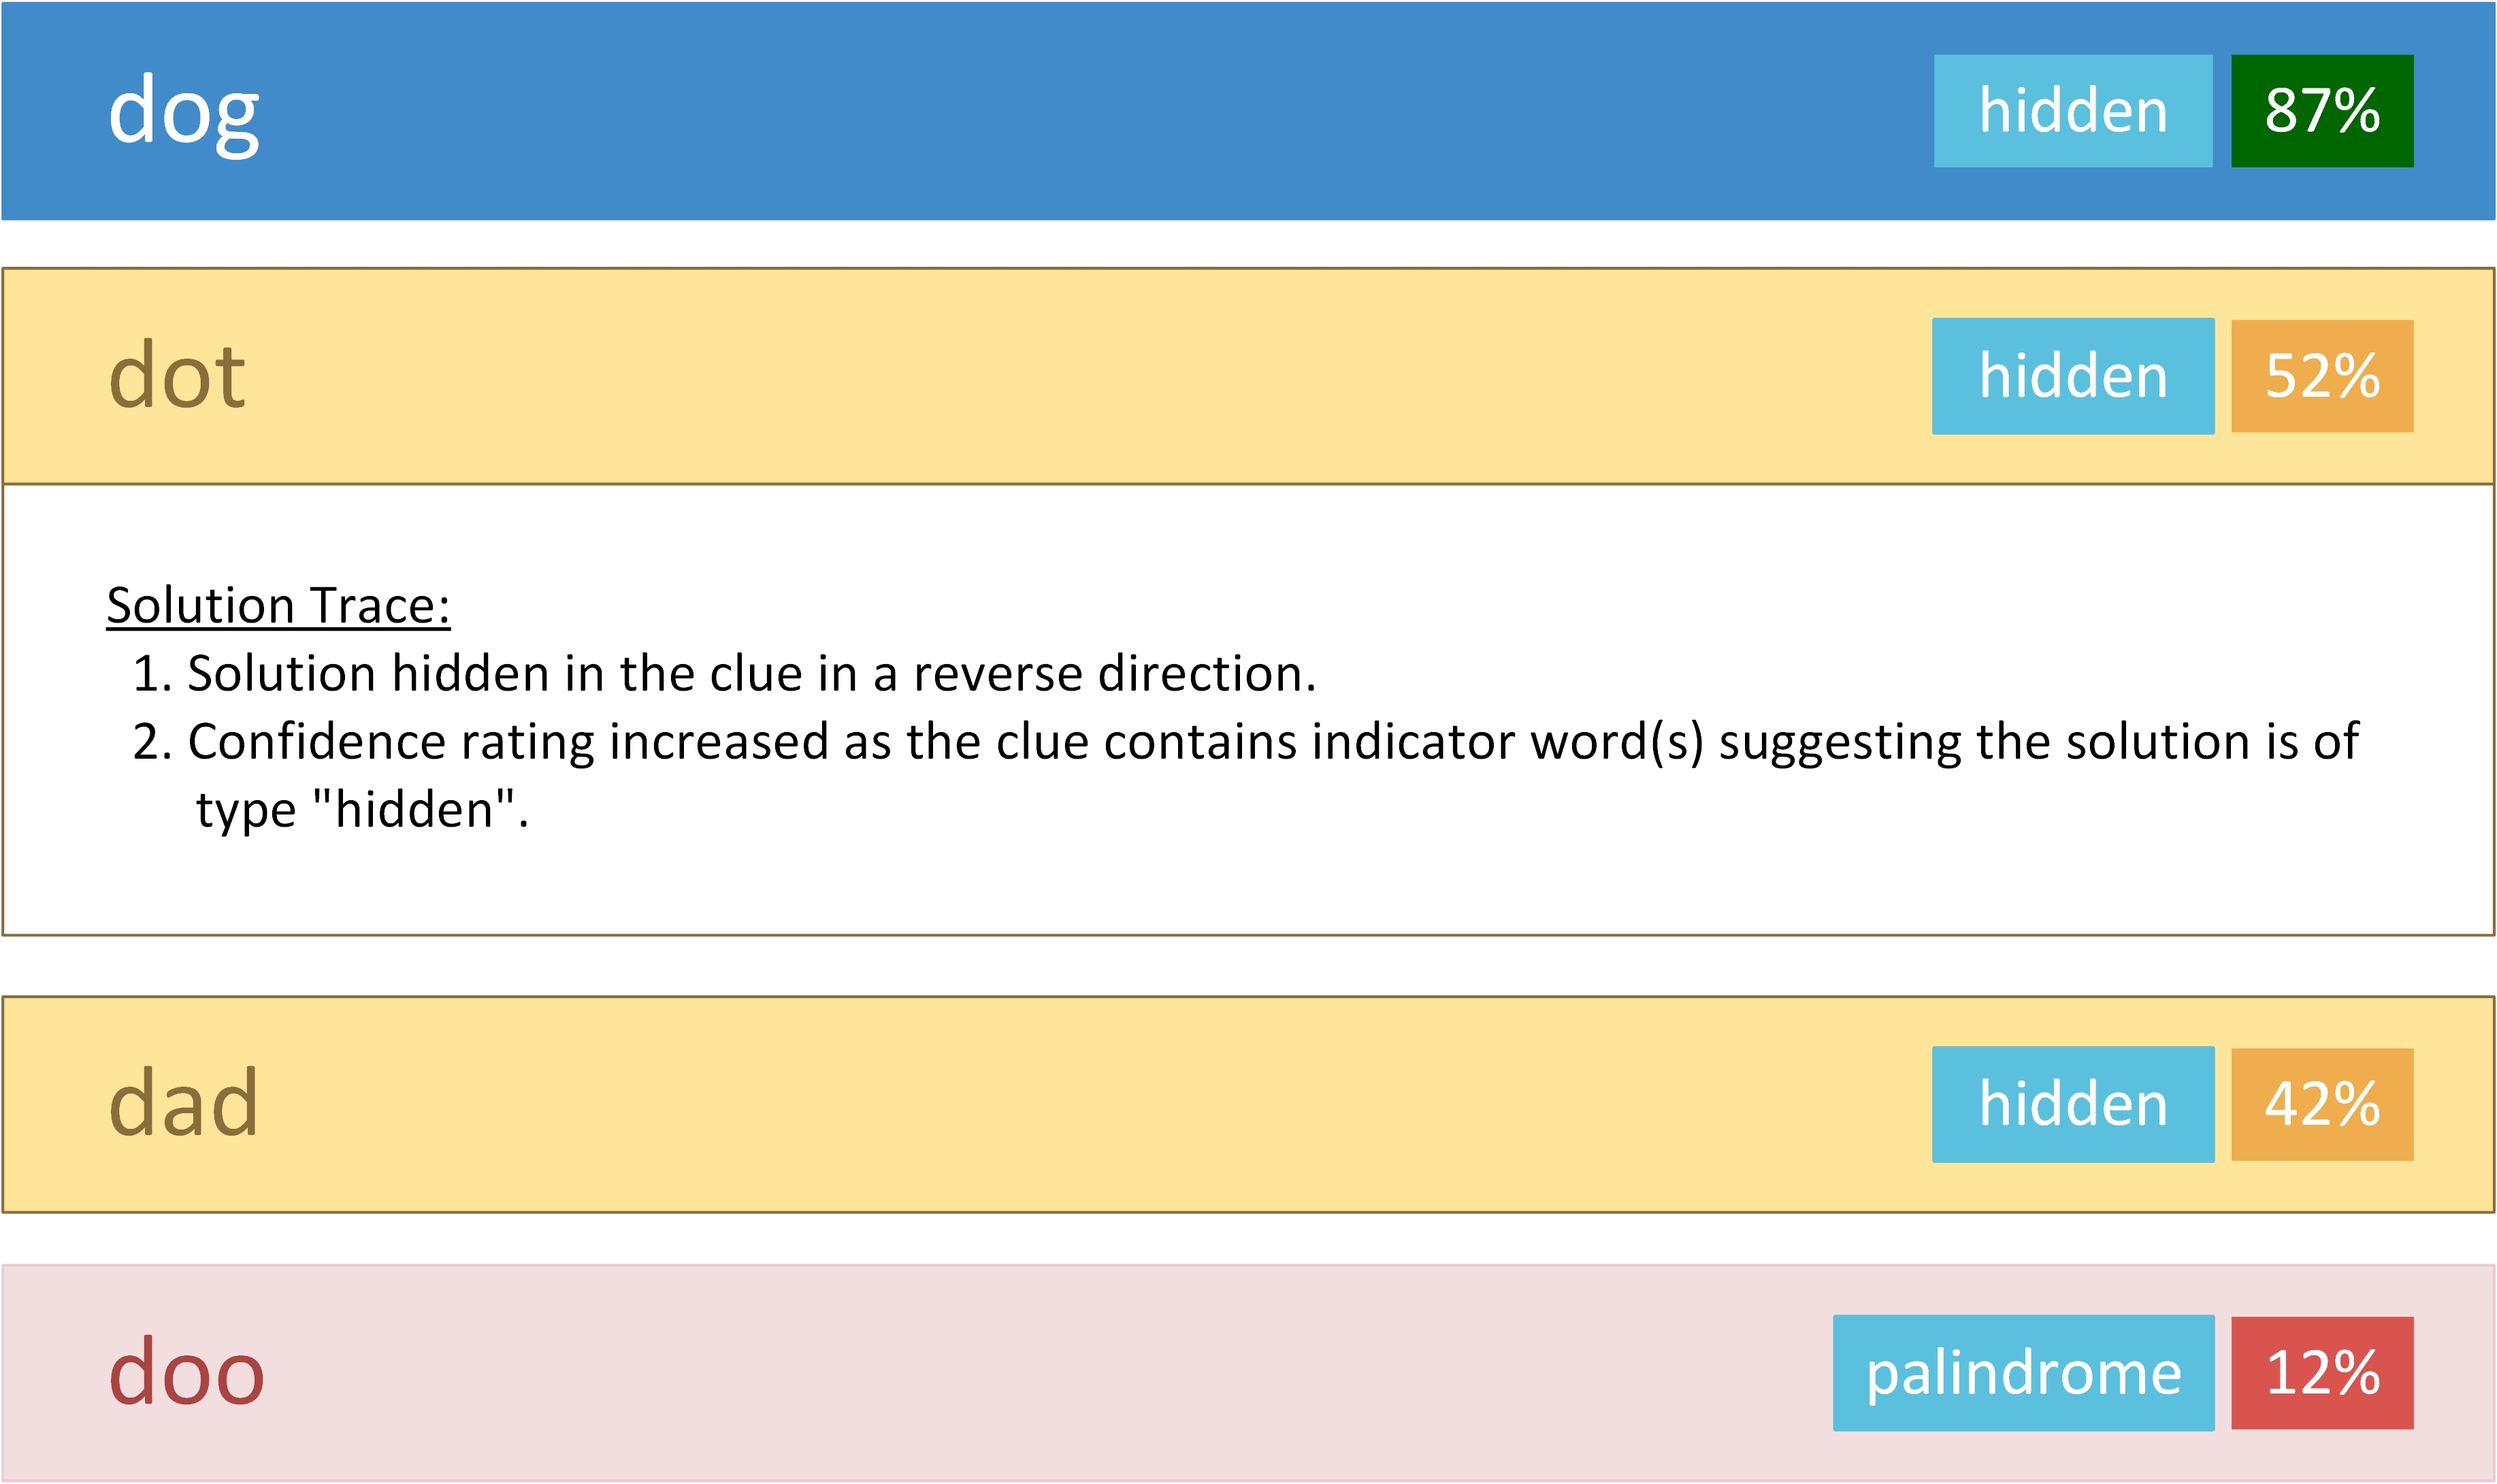
\includegraphics[width=0.8\textwidth]{design/ui/results_secondary.jpg}
  \caption{Results list displaying alternative solutions}
  \label{fig:results_secondary}
\end{figure}


% Servlet Development Details
\newpage
%%%%
%% Developers :: Web Service & Servlets
%%%
\section{Web Service \& Servlets}
\label{sec:servlet}

The core system is wrapped around a RESTful web service, that allows users from
various devices to submit clues to be solved. Within this section both the web 
service and the servlet implementations will be discussed and presented.


%%%%
%% Implementation :: Web Service & Servlets :: Web Service
%%%
\subsection{Web Service}
\label{sub:servlet_web_service}

During the project analysis phase the decision was taken that the system's
functionality will be delivered via a web service. The web service was developed
using Java Enterprise Edition (Java EE) and Tomcat 7.

The main reason for using Java is that the web service could easily make use of
the various packages that are provided by the chosen natural language processing
library --- Apache OpenNLP also written in Java.

The web service has solely been produced using the Java EE platform and does not
use any additional frameworks or libraries such as Apache Axis. The reason being
is that the Java EE platform will run on any machine that is capable of running
the Java virtual machine without any additional configuration.

Although Apache Axis (for example) provides additional functionality in
configuring the web service, it was decided that the project was to focus upon
the solving of a clue. Therefore a `standard web service' setup would easily
meet the requirements of the project.

Another design decision was taken to ensure that the web service followed a
RESTful style of communication. The main reason for this is that some of the
target devices (i.e. mobile and tablet platforms) do not support SOAP based
communication without additional plug-ins. RESTful web services also provide a
number of advantages over their SOAP-based counter parts, as was highlighted
within the research section.


%%%%
%% Implementation :: Web Service & Servlets :: Servlets
%%%
\subsection{Servlets}
\label{sub:servlet_servlets}

The servlet design has been split across two classes --- \texttt{Servlet} and 
\texttt{Solver}.

The \texttt{Servlet} class extends the standard \texttt{HttpServlet} class and
provides common functionality whilst also providing a standardised base for all 
future system servlets.

The \texttt{Servlet} class is able to deduce if a given request is from a JSON,
XML or an Ajax background. For example, if a client was to make a request to the
web  service through a web browser utilising an Ajax request, then the 
\texttt{isAjaxRequest} method would return \texttt{true}. For illustrative 
purposes the \texttt{isAjaxRequest} method is shown below in listing 
\ref{isAjaxMethod}.

\begin{lstlisting}[caption={isAjaxMethod deduces if a request was made by AJAX},
                   label=isAjaxMethod]  
  protected boolean isAjaxRequest(HttpServletRequest request) {
    String ajax = request.getHeader("x-requested-with");
    return ajax != null && ajax.toLowerCase().contains("xmlhttprequest");
  }
\end{lstlisting}

The servlet also contains two customised methods -- one to handle errors, and 
the other to handle a good response -- that are able to send a response back to 
the requesting client based upon a number of factors.

For example the methods are able to convert the return data into either XML or 
JSON depending upon what the client has asked for. The \texttt{sendError} method
will also set the HTTP status code correctly, allowing the client to correctly 
authenticate the response.

Finally the \texttt{Servlet} class overrides the \texttt{init} method, which 
is automatically called as part of the object construction. This method will 
initialise resources at servlet creation (i.e. first run-time within tomcat) 
rather than during the first call to the servlet. 

In doing this, Tomcat will take more time initially starting up, however the 
user will notice that their queries are dealt with much quicker. In this project
the \texttt{init} method has been used to initialise the various in-memory 
dictionaries and thesauri.

The second class is the \texttt{Solver} servlet and handles all requests that are
specifically for solving a given clue. The \texttt{Solver} servlet accepts both
GET and POST requests, with each requiring the clue, the length of the solution
and the solution pattern.

The \texttt{Solver} servlet upon receiving a request will validate the input 
parameters, based upon a number of criteria including presence checks and 
regular expressions. Listing \ref{isPatternValid} shows an example validation 
rule that will validate the solution pattern against a regular expression.

\begin{lstlisting}[caption={isPatternValid deduces if a given solution pattern 
                            is valid}, label=isPatternValid] 
 private boolean isPatternValid(String pattern) {
    // Pattern string regular expression
    final String regex = "[0-9A-Za-z?]+((,|-)[0-9A-Za-z?]+)*";
    boolean match = Pattern.matches(regex, pattern);

    // Pattern String must be present and of a valid format
    return isPresent(pattern) && match;
  }
\end{lstlisting}

In order for validation to pass, the solution pattern must not be empty and must
match to the regular expression shown in the above method.

The \texttt{Solver} servlet class will initialise the solving of a clue if the 
three inputs are deemed to be valid. The \texttt{solveClue} method will utilise 
the Clue manager class, that will handle the distributing of the clue to the 
various solvers. 

This has been designed so that the servlet and the solving processes are upon 
separate threads. This prevents Tomcat from freezing and allows it to handle 
requests from users.

Once all the solvers have finished executing, the \texttt{Solver} servlet will 
produce an XML document based upon the various elements. Once the XML document 
has been created, it will be sent back to the client as either XML or JSON.


% Core Package
\newpage
%%%
%% Development :: Core
%%%
\section{Core}
\label{sec:core}

Within this section the core package will be presented. The core package is the 
package that forms the heart of the system, and provides various base classes
that when instantiated will represent Clues, Solutions and Solution Patterns.


%%%
%% Development :: Core :: Clue
%%%
\subsection{Clue}
\label{sub:clue}

The clue class represents an individual cryptic crossword clue, and will 
maintain a list of possible solutions that have been computed. The Clue class is
a basic class, that essentially provides references to other aspects of solving 
a clue, such as the solution pattern (see subsection \ref{sub:solution_pattern}).

A clue is able to have a number of solutions, and hence each clue will house a 
SolutionsCollection, which is described in more detail in subsection 
\ref{sub:solution_collection}.

A clue will also have a solution pattern -- described in subsection 
\ref{sub:solution_pattern} -- which allows for potential solutions to be matched 
against an expected pattern.


%%%
%% Development :: Core :: Solution
%%%
\subsection{Solution}
\label{sub:solution}

The solution class implements the Comparable interface, which is a standard Java
interface that imposes ordering upon the object that implements it. It was 
decided that the solution class should implement the interface, so that 
solutions can be compared.

The comparing of solutions is perhaps one of the most common pieces of 
functionality that the system will be required to do. An example use case would
be comparing any number of solutions to deduce which is more likely to be 
correct answer.

Listing \ref{compareToSolution} shows the implemented compareTo() method found
within the Solution class.

\begin{lstlisting}[caption={compareTo() compares two solutions},
                   label=compareToSolution] 
  public int compareTo(Solution o) {
    int solutionCompare = solution.compareTo(o.getSolution());
    int confidenceCompare = -1
        * Double.compare(confidence, o.getConfidence());

    if (solutionCompare == 0) {
      // compare the actual solution text.
      return 0;
    } else if (confidenceCompare == 0) {
      // return a comparison of the solution text. 
      return solutionCompare;
    } else {
      // compare them based on their confidence.
      return confidenceCompare;
    }
  }
\end{lstlisting}

The above code will try to deduce which of the two solutions are closest to 
being correct. It does this by comparing their confidence ratings, to which 
every solution will have. If the solution is the same the 0 is returned, whist 
-1 or +1 returned depending upon which solution is closest to being correct.

As well as the housing the confidence rating, the solution class also houses the
solution trace. The solution trace is a List of steps that were taken in order 
to compute the solution. It is intended that the solution traces will help to 
teach the user how to complete similar clues in the future. 


%%%
%% Development :: Core :: Solution
%%%
\subsection{SolutionCollection}
\label{sub:solution_collection}

The SolutionCollection class extends the standard Java HashSet class utilising 
the Solution class as the element type. Although a HashSet can not guarantee the
order of the set, it can guarantee that no duplicates will be added to the set.
This decision was taken to ensure that the system is not dealing with large 
amounts of repetitive datasets, that will only harm the performance of the 
system as whole.

In order to get around the fact that the ordering of the set has not guarantee,
the system makes use the of fact that the element type -- Solution -- implements
the Comparable interface. This means that a copy of the current collection can 
be retuned in a sorted order if possible. This is illustrated in listing 
\ref{sortSolutions_SolutionsCollection}.

\begin{lstlisting}[caption={Method returns a new sorted collection},
                   label=sortSolutions_SolutionsCollection] 
  public Set<Solution> sortSolutions() {
    return new TreeSet<>(this);
  }
\end{lstlisting}

As both the TreeSet class and the HashSet both share the same parent class Set,
it is possible to cast the result of this method back to a SolutionCollection.

The SolutionCollection class overrides basic methods found within the HashSet 
class, such as \texttt{contains}, \texttt{add}, \texttt{addAll}, whilst 
providing additional functionalities, such as returning all solutions whose 
confidences are greater than (or less than) a given value.


%%%
%% Development :: Core :: Solution Pattern
%%%
\subsection{Solution Pattern}
\label{sub:solution_pattern}

The SolutionPattern class models the solution to a corresponding clue. For 
example if the clue is nine letters long, then the SolutionPattern class would 
provide information about the pattern of that solution using any given known 
characters.

The solution pattern is able to split a well-formed pattern and represent it 
as an in-memory object allowing for a faster clue matching process, in 
comparison to constantly trying to match a string.

An good example of the level of functionality available in this class is shown 
in listing \ref{filter_SolutionsPattern}.

\begin{lstlisting}[caption={Method returns collection of matched solutions},
                   label=filter_SolutionsPattern] 
public void filterSolutions(Set<Solution> solutions) {
  Collection<Solution> toRemove = new ArrayList<>();
  // For each proposed solution
  for (Solution solution : solutions) {
    // If it doesn't match the pattern, throw it out
    if (!match(solution.getSolution())) {
      toRemove.add(solution);
    }
  }
  solutions.removeAll(toRemove);
}
\end{lstlisting}  

The code snippet will match the given set of solutions --- often a 
SolutionCollection --- to the current object. A match can simply be described as
matching a solution pattern to a possible solution, for example `d??k' could 
match to `duck', `deck' or even `dork'.

This method is often used within the filtering down of potential solutions, and
thus ensures that the application is not dealing with too much data. In effect
this helps the application become more efficient when solving solutions. 

Obviously the efficiency of the matching process is directly linked to the 
number of known characters. If large number of known characters are given by the
user, then the total `search space' is dramatically reduced.

As an example there are about 308 million different letter combinations within a
six letter word ($26^6$) -- this refers to the arrangement of letters, and not 
`actual' words. If just one of those letters is known, this would be reduced 
down to 11 million different letter combinations ($26^5$), and knowing two 
letters would reduce it down to around half a million ($26^4$).


%%%
%% Development :: Core :: Manager
%%%
\subsection{Manager}
\label{sub:manager}

The Manager class manages the process of solving the given clue. The manager 
class heavily utilises the standard Java future interface, which is designed to
represents the result of asynchronous computation.

Listing \ref{distributeAndSolveClue} illustrates the distribution functionality 
that distributes a copy of all the necessary resources --- such as the clue 
and it's solution pattern -- and starts the computation upon various new 
threads (if available upon the system).

Each of the solvers are obtained dynamically via the plug and play system to 
which more information can be found within section 
\ref{sec:plug_and_play_architecture} on page \pageref{sec:plug_and_play_architecture}.
Once the solvers are obtained they are initialised. The initialisation process
simply creates a new object instance of the solvers, and starts them solving the
clue.

Once all solvers have finished, their computed solutions are added to an overall
solutions collection, which will ignore duplicate solutions as explained in 
section \ref{sub:solution_collection}.

Each of the solutions will have their confidences adjusted based upon how 
`correct' the solution is.

\begin{lstlisting}[caption={Method to distrbute the clue out to all solvers},
                   label=distributeAndSolveClue] 
public SolutionCollection distributeAndSolveClue(Clue clue) {
    // This will hold the solvers to be run at runtime
    Collection<Solver> solvers = getSolversFromClasses(clue);
    // This will hold the returned data from the solvers
    Collection<Future<SolutionCollection>> solutions = initiateSolvers(solvers);
    // This will hold all solutions that have been returned
    SolutionCollection allSolutions = new SolutionCollection();
    // Now we need to 'unpack' the SolutionCollections
    for (Future<SolutionCollection> future : solutions) {
      try {
        allSolutions.addAll(future.get());
      } catch (InterruptedException | ExecutionException e) {
        e.printStackTrace();
      }
    }
    // Adjust confidence scores based on category matches
    Categoriser.getInstance().confidenceAdjust(clue, allSolutions);

    return allSolutions;
  }
\end{lstlisting}  


% Plug & Play Architecture
\newpage
%%%
%% Development :: Plug and Play Architecture
%%%
\section{Plug and Play Architecture}
\label{sec:plug_and_play_architecture}



% Solvers
\newpage
%%%
%% Development :: Solvers
%%%
\section{Solvers}
\label{sec:solvers}

A Feasibility Study was created to attempt to predict the difficulty of specific
 clue types and their regularity in cryptic crosswords. All seventeen clues
 types were analysed in order to plan which would be implemented in each
 iteration of the implementation process. The first iteration involved Hidden,
 Anagram, Acrostic and Pattern as they all had a low difficulty. The next iteration
 involved Homophones, Palindromes, Double Definition and Spoonerisms to step
 up the difficulty of the algorithms. Finally, the last solvers to be implemented were
 Charades, Deletions, Containers and Reversals as they were seen as the most
 beneficial to implement in the time left for the project. 

Therefore, with the additional reason of a time limit,  Purely Cryptic and
 \& lit clue types were not implemented due to their high difficulty and Substitutions,
 Shifting and Exchange clue types were not implemented due to their rarity.

%%%%
%% Implementation :: Solvers :: Hidden
%%%
\subsection{Hidden}

When investigating the Hidden clue type, it was found that the answer to the clue 
would be within the clue itself. For example:

Creamy cheese used in apricot tart.

 
ANSWER: Ricotta

In the clue above the answer 'ricotta' is hidden within the two words 'apricot tart'.
The algorithm takes the clue as a whole, without spaces, and then uses the substring method 
within Java to find all possible hidden words (as the Hidden clue type can also hide words
 in reverse, the clue is also passed in reverse). It does this by taking the index of
 the for loop and length of the solution as boundaries. The following piece of code 
illustrates how all possible solutions are found (without additional solution trace
functionality):

\begin{lstlisting}
 int index;
 for (index = 0; index <= limit; index++) {
	Solution s = new Solution(clue.substring(index, index + totalLength), NAME);
	solutions.add(s);
 }
\end{lstlisting}

For the above clue, where limit is equal to seven because 'ricotta' is seven letters 
long, the first five iterations will add the following solutions to the list; 'creamyc', 
'reamych', 'eamyche', 'amychee', 'mychees'. Eventually, the loop will pick up 
'ricotta' and add it to the solution list. From the output gained in the first five 
iterations it is apparent that a lot of invalid solutions are added to the list, therefore
a number of steps are also implemented to eliminate invalid solutions.

Once all possible solutions have been found, they are all checked to make sure they are
not words from the original clue. For example, 'apricot' is seven letters long and will 
have been picked up through the algorithm, however it is not a hidden word and therefore 
not a valid solution. 

Next, the solutions are checked against the pattern provided. This means if the user 
has input known letters or there are spaces in the end solution but the solution being 
checked does not match these requirements, these solutions are removed. 

Finally, all solutions are checked against the dictionary to determine whether they 
are valid words. The solutions that are left are then returned to the user.   

%%%%
%% Implementation :: Solvers :: Anagram
%%%
\subsection{Anagram}

%%%%
%% Implementation :: Solvers :: Acrostic
%%%
\subsection{Acrostic}

%%%%
%% Implementation :: Solvers :: Pattern
%%%
\subsection{Pattern}

%%%%
%% Implementation :: Solvers :: Homophone
%%%
\subsection{Homophone}

%%%%
%% Implementation :: Solvers :: Palindrome
%%%
\subsection{Palindrome}

%%%%
%% Implementation :: Solvers :: Double Defintion
%%%
\subsection{Double Defintion}

%%%%
%% Implementation :: Solvers :: Spoonerism
%%%
\subsection{Spoonerism}

%%%%
%% Implementation :: Solvers :: Charade
%%%
\subsection{Charade}

%%%%
%% Implementation :: Solvers :: Deletion
%%%
\subsection{Deletion}

%%%%
%% Implementation :: Solvers :: Container
%%%
\subsection{Container}

%%%%
%% Implementation :: Solvers :: Reversal
%%%
\subsection{Reversal}

% Resources
\newpage
%%%
%% Development :: Resources
%%%
\section{Resources}
\label{sec:resources}

There are a number of resources which were needed to aid with solving 
the various clue types. As a lot of the solvers shared most of the resources 
a design decision was made to keep the resources in their own package for 
all solvers to access them as and when they need to.


%%%%
%% Development :: Resources :: Abbreviations
%%%
\subsection{Abbreviations}

Some clue types, for example the `Charade' clue type, require the knowledge 
of the different abbreviations that come with certain words. To provide this 
knowledge a file was found with a list of words and abbreviations in JSON 
format (JavaScript Object Notation). 

Listing \ref{abbr} illustrates the way in which the abbreviations for `quiet' 
are displayed in the file:

\begin{lstlisting}[caption={A sample of the abbreviations file},
                   label=abbr]  
 "quiet": [
  "p", 
  "pp", 
  "sh", 
  "mum"
 ], 
\end{lstlisting}

The Abbreviations class reads in all the possible abbreivations from the file 
at run time and stores them within a map which includes the word to get the 
abbreviations for and it's abbreviations as a set. 

There are two ways in which abbreviations could be needed to solve a clue, 
one way is to retrieve abbreivations for one word and the other is to 
retrieve abbreviations for a phrase or a whole clue. 

The method to retrieve abbreviations for one single word simply returns the 
set of abbreviations for a given word (or key) in the map if it exists within the 
file. 

The method to get abbreviations for a phrase or a whole clue gets the
abbreviations for as many words as possible in the given clue. For example,
``help the medic'' will contain seven abbreviations for the word  medic. ``medal
for the medic'' will contain four abbreviations for medal and seven  for medic.
However, the clue ``master of ceremonies'' will return one  abbreviation which
matches the entire clue (i.e. ``master of ceremonies'').  The algorithm is
greedy, and will attempt to match the biggest String possible in the given clue.
This means it will match all of the String  ``master of ceremonies'' before
matching abbreviations for ``master''.

%%%%
%% Development :: Resources :: Dictionary
%%%
\subsection{Dictionary}

The dictionary is an essential resource for the solving of clues to 
programmatically determine whether a string of letters is a valid word. 
A text file was found with a list of words within it which is read into the 
Dictionary class when an instance is created.

Listing \ref{dict} illustrates simply how the words in the dictionary file are
displayed:

\begin{lstlisting}[caption={A sample of the dictionary file},
                   label=dict]  
abaci
aback
abacs
abactinal
abactinally
abactor
abactors
abacus
\end{lstlisting}

Once the file has been read in, there are a custom list of words to  exclude
from the dictionary and a list of words that need to be added  found from
solving particular clues.

One of the methods used regularly is the filtering method which removes any
words from a given collection that are not present in the dictionary. This is an
effective way to remove words that have being constructed by a solver algorithm
which are essentially just an assortment of letters which hold no identified
meaning.  A similar method is used to filter any prefixes passed in within a
collection that are  also not held in the dictionary.

When potential solutions have been found by a solver, it is necessary to ensure
the algorithm has returned solutions that fit the end solutions pattern.
Requirements  such as the length input by the user and any known letters input
by the user must  be adhered to. In the dictionary class there is a method which
gets all word matches  within the dictionary for a given solution pattern. As
with filtering solutions, there is  also a method to match up all words in the
dictionary that have the same prefix as  a prefix passed in.

There are also simple methods solvers can use to identify whether a single word
or a  phrase is contained within the dictionary simply by checking whether the
collection the  dictionary file has been read into contains the word or not.

%%%%
%% Development :: Resources :: Thesaurus
%%%
\subsection{Thesaurus}

For clue types which do not have the answer itself nested within it, it is
usually necessary  to take the clue words and find synonyms for them. This is
where the necessity for a thesaurus  applies to aid the algorithms in solving
clues. A thesaurus file was found which holds a vast number  of entries where
each word after the first word in an entry is a synonym of the first word.

Listing \ref{thes} illustrates how the words in the thesaurus file are displayed
with the example word `dank':

\begin{lstlisting}[caption={A sample of the thesaurus file for the word `dank'},
                   label=thes]  
dank,boggy,damp,dampish,dewy,fenny,humid,marshy,moist,muggy,
     rainy,roric,roriferous,sticky,swampy,tacky,undried,wet,
     wettish
\end{lstlisting}

As with the other resources the file is read in and stored within a collection,
this  time in the form of a map where the first word is stored within an entry
along with it's synonyms.

There are a wide range of different methods that can be used to retrieve a
different array  of synonyms from vague to specific. Below is a list of
functionality that has been written  to retrieve synoynms:

\begin{itemize}
  \item Obtain a list of ``synonyms of a word's synonyms'' to increase the 
        chances of finding the correct solution. These must match against a 
        supplied pattern. 
  \item Obtain a list of ``synonyms of a word's synonyms'' to increase the 
        chances of finding the correct solution. These must match a minimum and
        maximum length passed in for the synonym.
  \item Retrieve all single word synonyms of a given word with a maximum and 
        minimum length (because some synonyms can be more than one word long) 
  \item Retrieve all synonyms of a given word with no pattern or minimum or 
        maximum length
  \item Get the synonyms for as many words as possible in the given clue. For 
        example, in the clue ``help the medic'', look for synonyms of ``help the
        medic'', ``help the'', ``the medic'', ``help'', ``the'', ``medic''.
  \item Retrieve all synonyms in the same entry in the thesaurus as a given 
        word. This means to not only look at the first word of an entry for 
        synonyms, look through all entries and return every entry which contains
        a given word.
  \item Retrieve all synonyms in the same entry in the thesaurus as a given word
        which match against the given pattern.
  \item Check if a given potential solution found by a solver matches as a 
        synonym against any of the words present in the clue.
\end{itemize}


%%%%
%% Development :: Resources :: Homonym Dictionary
%%%
\subsection{Homonym Dictionary}

The `Homophone' clue type requires a resource for retrieving homonyms for words.
A file was found which lists words with a string representation of the words
pronunciation  and as with the other resources, the file is read in and stored
within a collection holding  the word and an list of the pronunciation split
into chunks. 

An additional collection  is formed which is essentially a reverse of the first
collection created. This allows pronunciations  to be looked up faster. For
example, looking up the pronunciation ``HH AH0 L OW1'' will return  ``hello''.
This saves having to iterate the entire homophone map to search for words with
the same pronunciation.

Listing \ref{homonym} illustrates how the words in the homonym dictionary file 
are displayed with the example word `hello':

\begin{lstlisting}[caption={A sample of the homonym dictionary file for the word
                            `hello'}, label=homonym]  
HELLO  HH AH0 L OW1
\end{lstlisting}

The class allows the algorithm to retrieve the pronunciation of a given word as
well as  get words which share the same pronunciation as the supplied word. This
only works for words  which share the exact same pronunciation.


%%%%
%% Development :: Resources :: Categoriser
%%%
\subsection{Categoriser}

Some algorithms for certain clue types require indicators to determine how to
generate  the end solution. For example, the `Container' clue type requires an
indicator to identify  which word is the container word and which word is to be
contained. For the purpose of  providing a confidence score for an end solution,
indicators can also be used. As the clue  is passed to all solvers, it is
possible that two solvers may return the same answer back to the user.  By using
the indicator file associated with the clue type it is possible to assign a
higher rating  to a solution from a solver if the clue has an indicator within
it from the associated file.

To provide faster access to the indicators for each clue type, the files listing
the indicators  are read in and stored within a map in the Categoriser class
with the name of the clue type  and a collection of the indicators.

One use of the Categoriser class is to retrieve the indicators simply by passing
in a clue type.  Another, is the functionality to remove the indicator from a
clue to potentially speed up a solver  algorithm by removing extra unnecessary
checking on an indicator word.

Listing \ref{removing} illustrates how the indicator is removed from the clue:

\begin{lstlisting}[caption={Removing the indicator from the clue},
                   label=removing]  
 public String removeIndicatorWords(String c, String type) {
	// Remove any punctuation
	String clue = WordUtils.normaliseInput(c, false);
	// The indicator words for the given type have to be present
	if (indicators.containsKey(type)) {
		for (String i : indicators.get(type)) {
			if (clue.contains(i)) {
				// Only remove the first match
				clue = clue.replace(i, "");
				break;
			}
		}
	}
	// Remove any double spaces, etc...
	return WordUtils.normaliseInput(clue, false);
 }
\end{lstlisting}

The code above uses another class to remove any punctuation from the clue
itself, then it checks to see if the clue type has an entry within the map
storing all  the indicators. If a word in the clue matches an indicator in the
indicator file, it is  removed and the modified clue is returned.

As mentioned, the Categoriser class can also boost the confidence of a solution
if  it contains an indicator within the clue that is featured in the indicator
file.

Listing \ref{conf} illustrates how the confidence is boosted using indicators:

\begin{lstlisting}[caption={Boosting the confidence of a solution},
                   label=conf]  
 public void confidenceAdjust(Clue c, SolutionCollection solutions) {
	Collection<String> matchingTypes = getMatchingClueTypes(c);
	for (String clueType : matchingTypes) {
		for (Solution s : solutions) {
			if (clueType.equals(s.getSolverType())) {
				double confidence = Confidence.multiply(s.getConfidence(),
						Confidence.CATEGORY_MULTIPLIER);
				s.setConfidence(confidence);
				s.addToTrace("Confidence rating increased as the clue contains indicator
                      word(s) suggesting the solution is of type \"" + 
                      clueType + "\".");
			}
		}
	}
 }
\end{lstlisting}

The first line of code in the previous method calls another method to retrieve  a
list of clue types that have an indicator in the associated indicator file which
matches a word  within the clue passed in. Then, all the solutions found from
all the solvers for the clue are passed in and are matched against the clue types that
have been found and if the solver and the solution has come  from matches a clue
type found, the confidence is boosted using a method in the Confidence class.


% Utilities
\newpage
%%%
%% Development :: Utilities
%%%
\section{Utilities}
\label{sec:utilities}

